\documentclass[../tech_report_1.tex]{subfiles}
\graphicspath{{img/}{../img/}}
\begin{document}

\section*{Spherical k-means clustering}

Spherical k-means clustering the same idea, but with points on a sphere.
We investigated a MATLAB implementation by Nguyen\cite{nguyen2008gene,nguyen_spherical_clustering},
which required a mean-and-norm-normalized dataset located on a hypersphere.
Important aspects of this implementation include:
\begin{itemize}
\item When there exists an empty cluster, the largest cluster is split
\item Use the dot product as ``negative distance'', which leverages the
fact that observations are unit vectors on the hypersphere
\item Use the normalized sum of observations as a centroid/mean, which leverages
the fact that observations are unit vectors on the hypersphere. Note
that this fails on pathological cases where the sum of observations
is zero.
\end{itemize}

\subsection*{Our investigation}

In order to test how well the spherical k-means clustering algorithm
worked, we constructed a random data set using the Von Mises distribution
random sampling function from the MATLAB Circular Statistics Toolbox\cite{circstats}.
We constructed 70 clusters of 10 points each, using random points
on the sphere as means and with $\kappa=100$, and then applied the
spherical k-means clustering and visualized the results on the unit
three dimensional sphere, color coded for each cluster and with estimated
means labeled as red $X$'s and true means labeled as black $X$'s.

\begin{figure}


\caption{Plot of 70 clusters and means on a 3-D sphere}


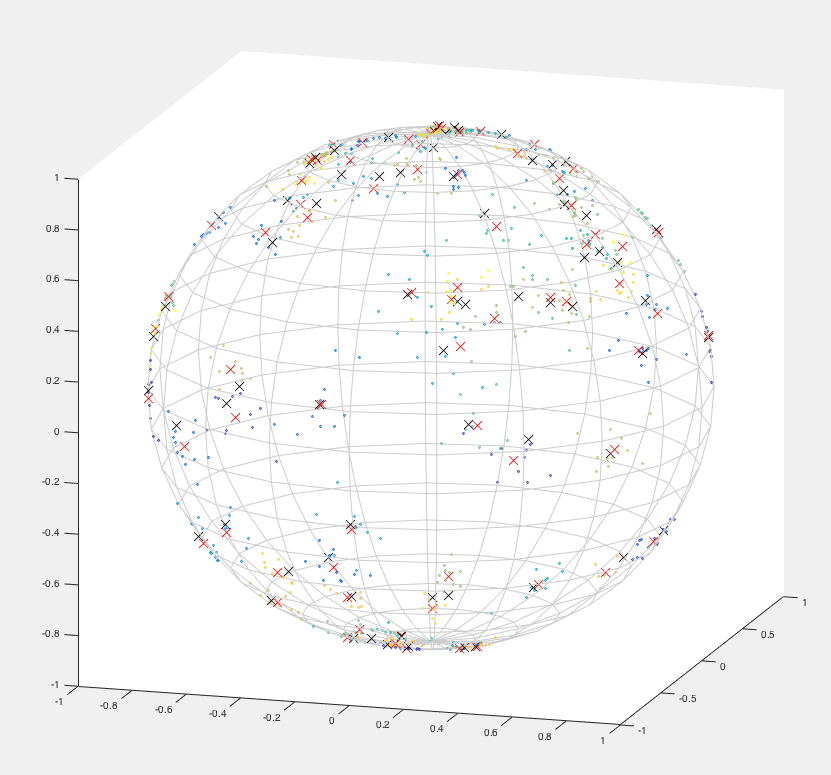
\includegraphics[width=1\textwidth]{sphere_points_70_clusters}
\end{figure}


\begin{figure}
\caption{Plot of 10 clusters and means on a 3-D sphere}


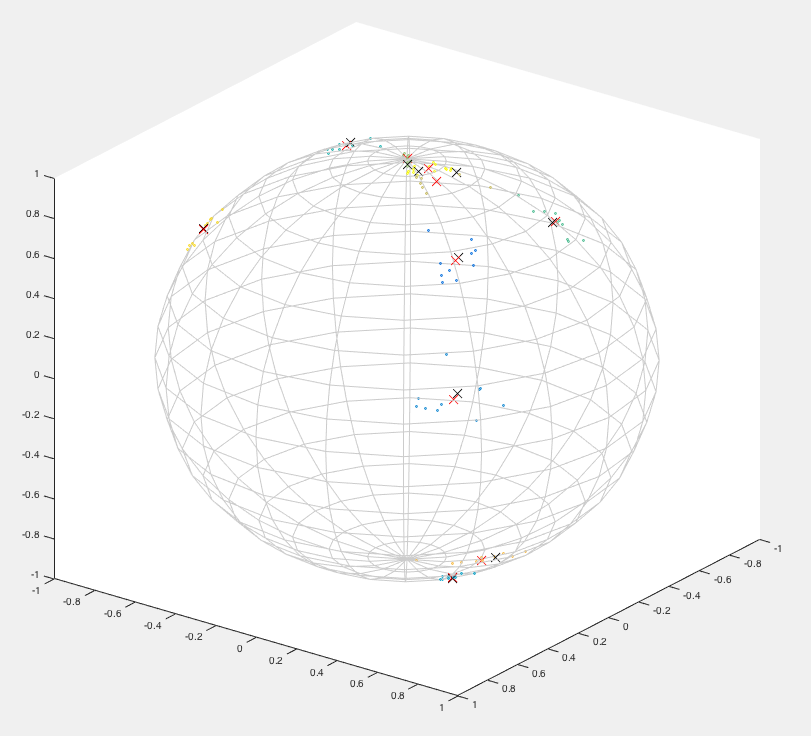
\includegraphics[width=1\textwidth]{sphere_points_10_clusters}
\end{figure}


\end{document}
